\pagestyle{headings}
\pagenumbering{arabic}
\chapter{Introduction}
\label{chapter:introduction}
\section{DNA methylation} 
\label{section:DNAMeth} 
Epigenetics is the name of the science that studies the heritable information not relying on changes in the DNA sequence and influencing the organisms phenotype. There exist two kinds of epigenetic modifications: Chromatin and DNA modifications. Chromatin is the three-dimensional arrangement of DNA and a histone protein. The modification of Chromatin is performed by binding of an amino group or RNA.\cite{Epigenetics}\\

The most common DNA modification is the addition of one methyl group to the fifth position in the cytosine ring of DNA. Methylation occurs mainly at \acp{CpG}, where a cytosine nucleotide (C) is followed by a guanine nucleotide (G) in the DNA sequence.\cite{DNAMethylation} Whereas the majority of CpGs in mammals are methylated, so called \ac{CGI} are rather unmethylated. The \acp{CGI} are associated to gene regulation as they are often located at the promoter region of genes. Hereby, methylation inhibits the gene expression; ensuring that changes in the methylation pattern of the DNA are effecting diseases like cancer.\cite{Handbook} Hypomethylation of repeat elements for example results in an unstable DNA and may increase the risk of cancer; as also the hypermethylation of cancer suppressor genes.\cite{DNAMethylation} Finally, DNA methylation is responsible for genomic imprinting and X-chromosome inactivation, whereby one of the two alleles respectively is transcribed and the other inactivated by methylation. Dysregulation may contribute to diseases like Prader-Willi syndrome, Angelman syndrome and cancer. \cite{Walter}\\

The transfer of the methyl group to the DNA is performed by \acp{DNMT}. Five different \acp{DNMT} are distinguished in mammals: DNMT1, DNMT2, DNMT3A, DNMT3B and DNMT3L.\cite{DNAMethylation}\\
DNMT1 is known as maintanance methyltransferase as its activity is associated with the DNA replication process. Thereby, not only the DNA of the cell is transmitted from one cell generation to another, but also the methylation patterns. DNMT1 has a preference for hemimythelated DNA, which means that one of the opposite \acp{CpG} is methylated and the other unmethylated. Subsequently, DNMT1 transfers the methylation by methylating the positions on the daughter strand that are methylated at the same position on the parental strand.\cite{DNAMethylation}\newline
DNMT2 is negligible if human DNA methylation is considered, because it methylates small RNA at the anticodon loop.\cite{DNMT2}\newline
DNMT3A and DNMT3B are de novo methyltransferases, which work during the early embryonic development to synthesize new methylations. Hereby, the enzymes do not show any preference neither for hemi- or unmethylated DNA nor for a DNA-strand. In other words, DNMT3A/B may add a methyl-group to any non-methylated \ac{CpG} at any DNA-strand. DNMT3L does not catabolize methylation, but increases the binding ability of DNMT3A/B and thus is required for establishing genomic imprinting.\cite{DNAMethylation}\newline
The loss of one of the methyltransferases leads to embryonic lethality.\cite{DNAMethylation}\\

So far a lot is known about the function of \acp{DNMT}, but some properties still remain unexplained:
\begin{itemize}
\item Why and where do the \acp{DNMT} bind?
\item On which conditions does the methylation event depend?
\item Which enzymes are able to methylate multiple \acp{CpG} in a row without deassociating from the DNA?
\item How much de novo and maintenance methylation do DNMT1 and DNMT3A/B perform?
\end{itemize}

To study the function of \acp{DNMT}, a computational model is designed and fitted using real biological data. These models are based on Markov models.

\section{Markov models} 
\label{section:MM}
A discrete-time Markov model is a stochastic model that fulfils the Markov property. If the next state can only be determined by the current state and not by the previous one, a chain holds the Markov property.\\

A \textbf{Markov chain} is the simplest Markov model. This chain is a sequence of variables $X_1, X_2, ...$ whose outcomes are random, so called \textbf{\acp{RV}}. Each \ac{RV} has a number of possible outcomes, the state space. Given a set of states $S = \{s_1, ..., s_n\}$ with transients between the states, $p_{ij}$ is the transition probability of $s_i$ to $s_j$. And P of size $|S|\cdot|S|$ is the transition matrix containing the transition probabilities between all states.\newline
Let $X_0$ be the initial distribution of the chain X s.t. $\sum_{x \in X_0}{x} = 1$, then $X_1 = X_0 * P$ is the distribution of X at time t=1. We call $\pi$ the \textbf{equilibrium distribution}; the distribution of X that does not change from one time step to another or formally: $\pi * P = \pi$.\\
%characteristics of Markov Chain? Ergodic...
\textbf{\acp{HMM}} are an extension of Markov chains. There are two kinds of states in this model; hidden states S and observable output states O. Similarly, there is a transition probability matrix between the states in S and a matrix of output probabilities B between the hidden and the output states.\newline
This model is used, when there is information about the output of a process, but no knowledge about the states of the system.\\
%Viterbi?

\section{Bayesian statistics} 
\label{section:Baystat}

\section{Problem} 
\label{section:Problem}
In the context of \acp{DNMT}, Markov models are used to simulate the function of the enzymes, making use of results from biological experiments. Here, few is known about the properties of methyltransferases, but the methylation patterns before and after the catabolism of the \acp{DNMT}. Each methylation state (unmethylated, hemimethylated, methylated) of one \ac{CpG} is an output state, whereas the binding state of the \ac{DNMT} at each \ac{CpG} is a hidden state. Thus the traversing probabilities between the hidden states P are equal to the probabilities of the \acp{DNMT} to bind/fall of and the output probabilities represent the different methylation probabilities:\newline
\begin{align}
O_i := \text{methylation state of CpG i}\\
O_i = \left\{
\begin{array}{ll}
0 & \text{unmethylated} \\
1 & \text{hemimethylated} \\
2 & \text{hemimethylated} \\
3 & \text{unmethylated} \\
\end{array}
\right.\\
S_i := \text{binding state of DNMT at CpG i}\\
S_i = \left\{
\begin{array}{ll}
0 & \text{unbound} \\
1 & \text{bound} \\
\end{array}
\right.
P := \text{probability of DNMT to change binding state}\\
B := \text{methylation probabilities}\\
\end{align}
Figure \ref{fig:fig} shows the four kind of methylation patterns.\\
\begin{figure}
\begin{subfigure}{.5\textwidth}
\centering
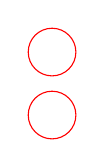
\begin{tikzpicture}
  \draw[red](0,0)circle(2ex);
  \draw[red](0,-0.8)circle(2ex);
\end{tikzpicture}
\caption{}
\label{fig:sfig0}
\end{subfigure}%
\begin{subfigure}{.5\textwidth}
\centering
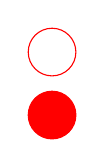
\begin{tikzpicture}
  \draw[red](0,0)circle(2ex);
  \draw[red, fill=red](0,-0.8)circle(2ex);
  \end{tikzpicture}
  \caption{}
  \label{fig:sfig1}
\end{subfigure}
\begin{subfigure}{.5\textwidth}
\centering
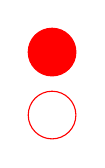
\begin{tikzpicture}
  \draw[red, fill=red](0,-0.2)circle(2ex);
  \draw[red](0,-1)circle(2ex);
  \end{tikzpicture}
  \caption{}
  \label{fig:sfig2}
\end{subfigure}
\begin{subfigure}{.5\textwidth}
\centering
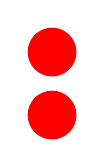
\begin{tikzpicture}
  \draw[red,fill=red](0,-0.2)circle(2ex);
  \draw[red,fill=red](0,-1)circle(2ex);
  \end{tikzpicture}
  \caption{}
  \label{fig:sfig3}
\end{subfigure}
\caption{Kind of methylation patterns; each figure shows two opposite CpGs on the parental and the daughter strand; each circle represents one CpG; plane red circles are methylated CpGs; (a) unmehtylated, (b) hemimethylated (upper strand unmethylated, lower strand methylated), (c) hemimethylated (vice versa), (d) fully methylated CpGs}
\label{fig:fig}
\end{figure}
Given the output sequence, we are able to determine the most likely sequence of S. Moreover, P and B can be reconstructed by computer simulation of the \ac{DTMC}. $One kind of simulation is \textbf{\ac{MCMC}}.$\\

Recently, different models and computational approaches were studied in order to predict the methylation process. Here we present some of them.\\

\section{Related work} 
\label{section:RelWork} 